\chapter{Full DressCode Language Specifications}

\subsection{Interface Design}
 \begin{center}
\begin{figure}[h!]
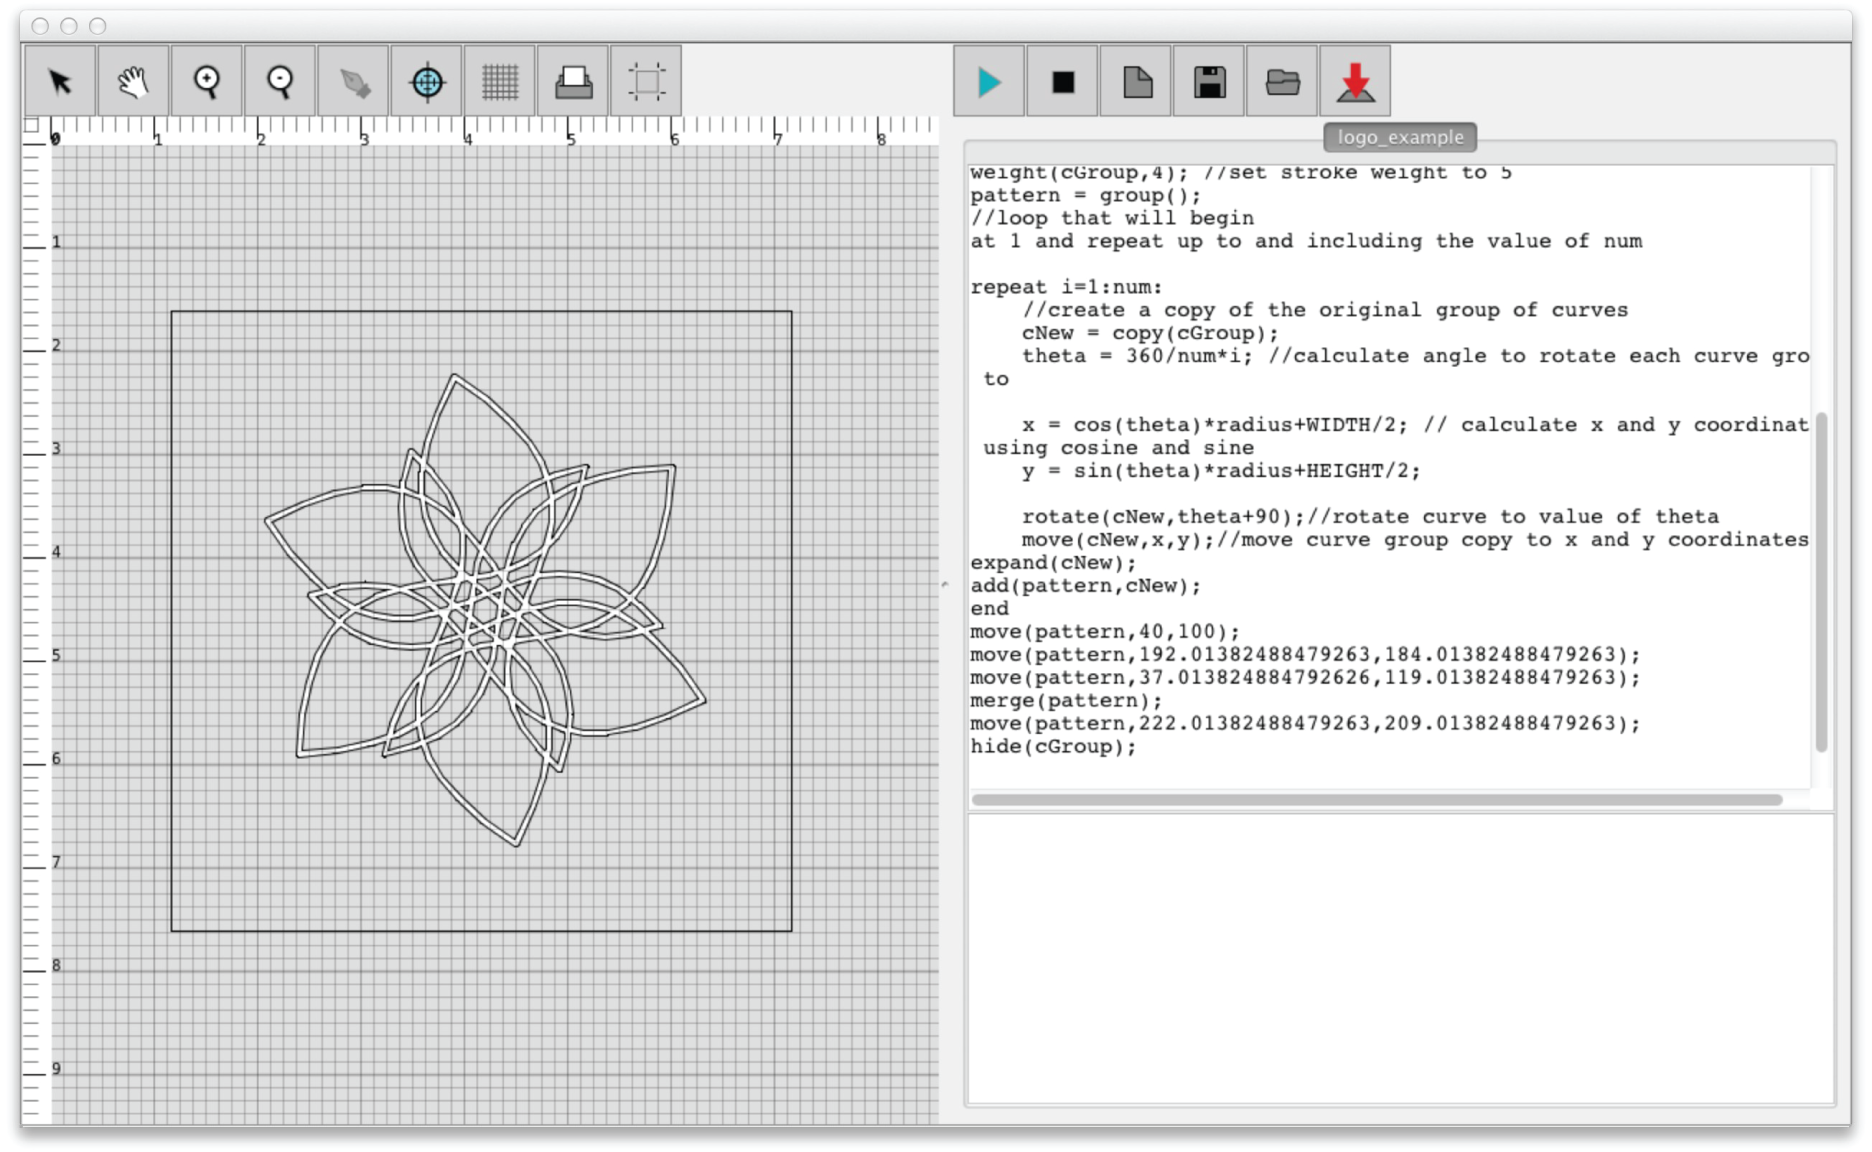
\includegraphics[width=6.5in]{images/dress_code_interface.png}
\caption{The DressCode interface}
\label{fig:dress_code_interface}
\end{figure}
\end{center}

The interface of DressCode is divided into two sections, a design panel and a coding panel. The divider between the two panels can be resized as needed. The coding panel contains a primary window for entering text, an output console for print output and error reporting and a row of buttons on the top. When the play button is pressed, the program in the code window is run and the resulting design is displayed in the design panel. The first version of DressCode ran the code each time the enter key was pressed or a new statement was completed, however we received many requests from our initial user tests for manual control of the run process. The stop button attempts to terminate programs that are taking too long to run.The following three buttons allow for the creation of new programs and the saving and opening of existing programs. The final button opens a dialog that enables the user to select an Scalable Vector Graphics (SVG) file to import into their script (the rationale for this is described in \ref{par:shape_transformation} section below.)

The design panel is primarily composed of the drawing canvas. The drawing canvas has a set of rulers and a grid, along with a black rectangle in the center which serves as the drawing board. The drawing board defines a reference for the coordinate system of the canvas, with the upper left hand corner corresponding to (0,0) in cartesian coordinates. Designs can be drawn on any part of the canvas, including outside the drawing board, however the exported designs file-dimensions will always correspond to the size of the drawing board. The right-most button in the design panel allows for the specification of the units of the project, and the resizing of the drawing board. The print button opens a dialog that allows the user to export their current design in a vector format. I experimented with various vector file formats including DXF, SVG and PDF, however for the time being, I settled on PDFs as they were compatible with the specific fabrication machines I intended to use in my workshops. 

The grid button allows the user to toggle between a grid in the units that correspond to the current units of the project (either millimeters or inches), pixels, or no grid. The target button allows the user to graphically select a set of coordinates and have them appear in the programming window as text, and can be used like an eyedropper for pixel coordinates. The plus and minus magnifying glasses and the hand tool are used to pan and zoom in and out of the screen.  Lastly, the arrow tool allows for design elements to be graphically selected and manipulated. After a design element is moved with the arrow tool, with the corresponding code for the move appears in the programing window. 

\subsection{Programing Language}
The DressCode programing language is interpreted with semantic functionality that is simulated through a Java-based library.  We relied on the ANTLR framework to generate the necessary lexing and parsing methods for the language, and developed the semantic functionality using java and the java openGL (JOGL). When a program is run in DressCode, the raw script is first tokenized and then parsed to generate an abstract syntax tree (AST). During this phase, all user-generated function definitions are stored in memory. If any parsing errors are encountered, they are output to the console as "compiler errors". Assuming the parse is successful, DressCode then walks the resultant AST and attempts to execute the semantic functionality of the program (figure:\ref{fig:interpreter_structure}.) After being executed, the resultant design is rendered on the display panel. Any runtime errors are displayed in the output console. For most programs, this process is instantaneous, however some programs with complex operations require several seconds to be executed. 
  \begin{center}
\begin{figure}[h!]
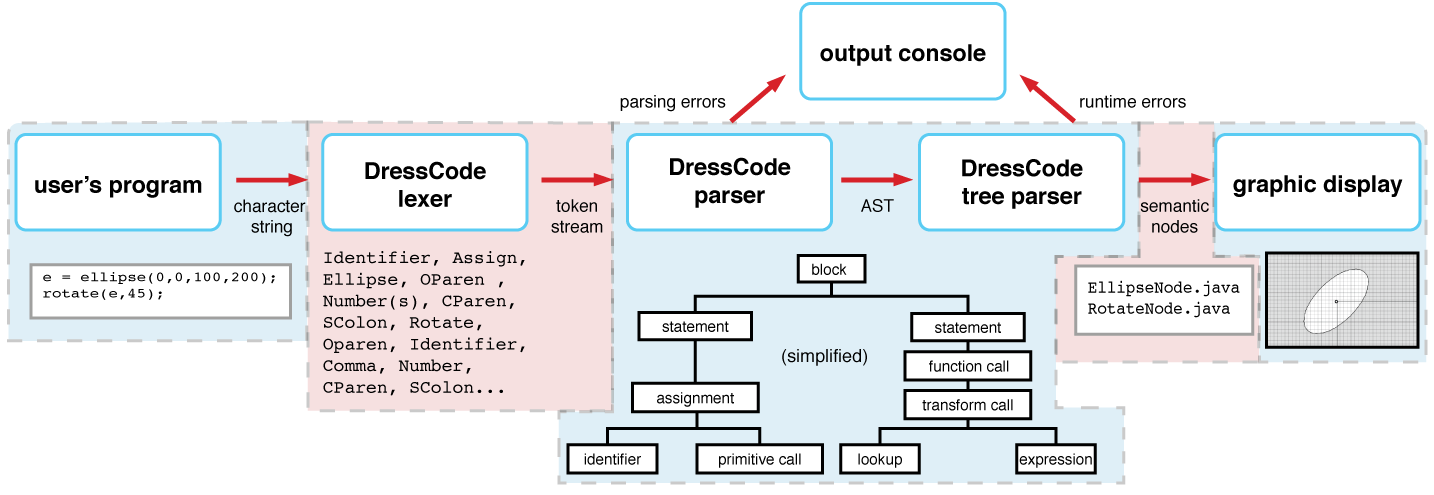
\includegraphics[width=6.5in]{images/interpreter_structure_horz.png}
\caption{Interpreter structure}
\label{fig:interpreter_structure}
\end{figure}
\end{center}
The language is imperative in nature, with statements being executed in the order in which they are read. The exception to this is user defined functions, which may be defined at any point in the program, and called before they are defined. Each statement in DressCode must be terminated by a semicolon. I spent some time experimenting with terminating statements with newlines, similar to whitespace sensitive languages like Python, as I thought this might be more conducive to novice use. Unfortunately, the implementation of selective whitespace recognition is a challenging task to define in a grammar, so while we were able to develop a version of DressCode that recognized statements terminated by a line break, it would have taken significant time to develop this functionality to a level of robustness appropriate for user testing. For the short term, we have opted for a syntax requiring semicolons, however we plan to continue to explore newline statement termination in the future. 

\subsubsection{Language Structure}
Here, I define some of the primary elements of the DressCode syntax and drawing API, and the rationale for their structure. A more thorough language reference is available on the DressCode wiki\cite{DressCodeWiki}.

 DressCode supports number, string, boolean, and drawable datatypes (figure \ref{fig:basic_datatypes}.) The first four of these types are relatively standard in comparison to conventional programing languages. Numbers include integers and floating point values. Strings include any sequence of characters enclosed in double quotations. Booleans have two possible values: true, and false. Drawables are a special type, discussed in detail in the API description below. DressCode also contains a list data structure, which can store multiple kinds of datatypes.
\begin{center}
%\begin{figure}
\begin{lstlisting}
myString = "hello";  //string
myNum = 10.4;  //number
numbermyBool = true;  //boolean
myList = [10,11,false,"world"];  //list with multiple data types
println(myList[3]); //prints world
\end{lstlisting}
%\caption{basic datatypes}
%\label{fig:basic_datatypes}
%\end{figure}
\end{center}

Variable identifiers in DressCode must begin with a letter which followed by 0 or more letters or digits. Variables can be initialized through assignment, or declared and assigned later in the program. All assignment in DressCode is dynamically typed, and variables can be assigned to datatypes that differ from their original assignment at any point. %(figure \ref{fig:variable_assignment}.)

\begin{center}
%\begin{figure}
\begin{lstlisting}
s1 = "hello";
s2 = "world";
s3; //variable without initial assignment

s3 = s1+" "+s2; 
println(s3); //prints hello world

n1 = 2;
n2 = 2.5;
println(n1+n2*10); // returns 27.0
\end{lstlisting}
%\caption{variable assignment.}
%\label{fig:variable_assignment}
%\end{figure}
\end{center}

The  language also contains support for basic expressions, as well as block statements, including conditionals, loops and user-defined functions. For mathematical expressions, standard order of operations is maintained, unless parentheses are introduced. All block statements are signified by a keyword followed by a colon, and terminated with the end keyword which is not followed by a semicolon.Conditionals are defined with the if keyword, and may an optional else clause and  zero or more else if clauses. %(figure: \ref{fig:conditionals}.)

\begin{center}
%\begin{figure}
\begin{lstlisting}
//if statement 
if 5<10:
println("true"); //prints true
end

//if statement with else if and else clause
i=10;
if i<10:
println("less than 10");
else if i==10:
println("equals 10"); //prints equals 10
else:
println("greater than 10");
end
\end{lstlisting}
%\caption{conditional definitions}
%\label{fig:conditionals}
%\end{figure}
\end{center}

There are two possible loop statements: repeat statements and while statements. Repeat statements begin with the repeat keyword and are followed by a the initialization: a variable identifier with a numerical assignment, followed by a colon and the test, a number that determines the point at which the repeat statement will terminate. By default, all repeat statements have an update value of 1, however this can be modified by following the test value with "add" and a 3rd value specifying the update condition. While loops are initialized with the while keyword and followed by a test condition.%(figure: \ref{fig:loops}.) 

\begin{center}
%\begin{figure}
\begin{lstlisting}
//repeat statement
repeat i=0:10:
ellipse(0,i*10,10,10); //draws a vertical row of 10 ellipses
end

//repeat with modified update condition
repeat i=0:10 add 2:
println(i); //will print 0,2,4,6,8
end

//while statement
c=0;
while c < WIDTH:
ellipse(c,10,20);
c = c+20;
end
//draws a row of ellipses that span the width of the canvas
\end{lstlisting}
%\caption{loop definitions}
%\label{fig:loops}
%\end{figure}
\end{center}

Finally, custom functions are defined with the def keyword, followed by an identifier and a set of parentheses containing 0 or more arguments separated by commas. The function block is terminated with the end keyword like all other block statements. Just like general assignments, functions arguments are dynamically typed. Functions, loops and conditionals all have their own scope and will prioritize identifiers based on that, however if they cannot locate an identifier within their own scope, they will look for it in the level above.
\begin{center}
%\begin{figure}
\begin{lstlisting}
//basic function defintion
def foo(a,b,c):
println(a+b+c);
end

//function call
foo(1,2,3);  //prints 6

//function with return statement
def bar(a,b,c):
return(a*b*c);
end

result = bar(4,5,6)); 
println(result);//prints 120
\end{lstlisting}
%\caption{loop definitions}
%\label{fig:loops}
%\end{figure}
\end{center}

\subsubsection{Drawing API}
 The API is organized around the creation and transformation of 2D shape primitives. By duplicating and manipulating these primitives in a structured manner, it is possible to generate complex and interesting designs from simple forms. The API is composed of three primary main categories, divided by functionality: shape primitives, shape transforms, shape booleans, math operations and property access. A selection of the primary methods from each of these categories is detailed in figure \ref{fig:api_table}. 

  \begin{center}
\begin{figure}[h!]
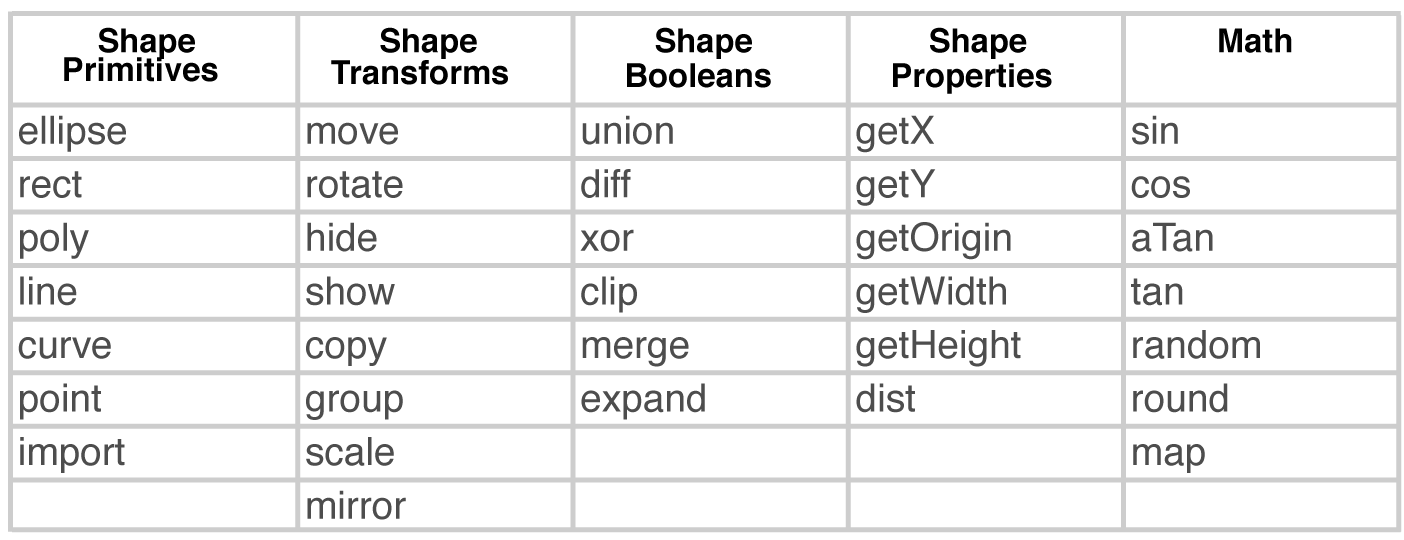
\includegraphics[width=6.5in]{images/api_table.png}
\caption{A selection of methods from the DressCode API}
\label{fig:api_table}
\end{figure}
\end{center}
\paragraph{Shape Primitives:}
DressCode shape primitives currently serve as the primary means of drawing (figure: \ref{fig:shape_primitives}.) The simplest primitive is a point, initialized two numerical parameters that denote the x and y coordinates. All closed-shape primitive methods (ellipses, rectangles and polygons) require an argument of either two x,y coordinates, or a point. This coordinate defines the origin of the shape and determines where  the shape will be drawn on the canvas. Ellipses and rectangles have an additional two optional parameters which specify width and height. If only two arguments are provided, the ellipse or rectangle will be drawn with a default width and height; if three arguments are given, the width and height will be the same. Polygons also have two optional parameters following the x and y origin coordinates, however they specify number of sides and length of each side, rather than width and height. Lines can be initialized either as four numerical values, specifying start and end x and y coordinates, two points, or as a vector, with a origin point,  a magnitude, and a heading in degrees. Curves are defined by a set of four points or eight coordinates, which determine the start, first control point, second control point and end point of a 4-point bezier curve. One other method of primitive generation was added in at the request of some of our early users: vector paths stored in Scalable Vector Graphics (SVG) format can be imported and drawn in the DressCode environment, and used in conjunction with primitive transformation and boolean methods.  

 \begin{center}
\begin{figure}[h!]
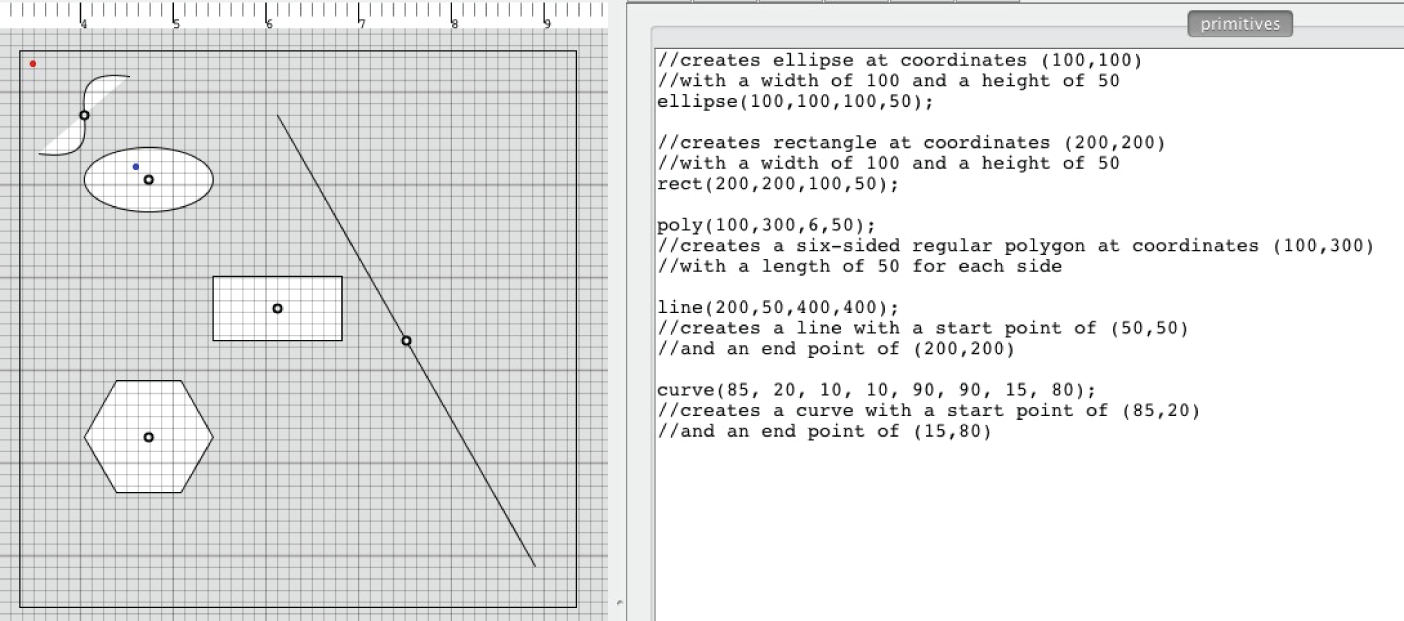
\includegraphics[width=6.5in]{images/primitives.png}
\caption{DressCode shape primitives with visible origins}
\label{fig:shape_primitives}
\end{figure}
\end{center} 

\paragraph{Shape Transformations:} \label{par:shape_transformation}
There is no required "draw" method for DressCode, as there are in many other graphics APIs, Instead all primitives are automatically drawn in the display panel in the order of their initialization, once the program has been run. In Soft Objects and Codeable Objects, when we required users to manually call draw method for any and all shapes in their program, they often forgot, and then had difficulty determining the reason why parts of their designs were not visible. 

Each shape primitive method returns an instance of the primitive it creates. A programmer can either create shapes with no reference as in figure \ref{fig:shape_primitives}, or they can assign them to an identifier at initialization, allowing them to reference and modify the shape later in the program. The shape transformation methods allow for a range of modifications to a shape, by passing a reference to the primitive the first argument, followed by different parameters for the modification, depending on the method (figure: \ref{fig:transformation}.) We began with a basic set of transformations, including move, rotate, methods that allowed for the modification of the stroke weight and color of the shape, and a hide method that prevented a primitive from being drawn. Based on our early user testing however, we gradually added in additional methods, based on what people wanted to do with their designs. This included a moveBy method, scale and mirroring functionality, a copy method, and an addition to the rotate method which allowed a shape to be rotated around a point other than its origin. 

 \begin{center}
\begin{figure}[h!]
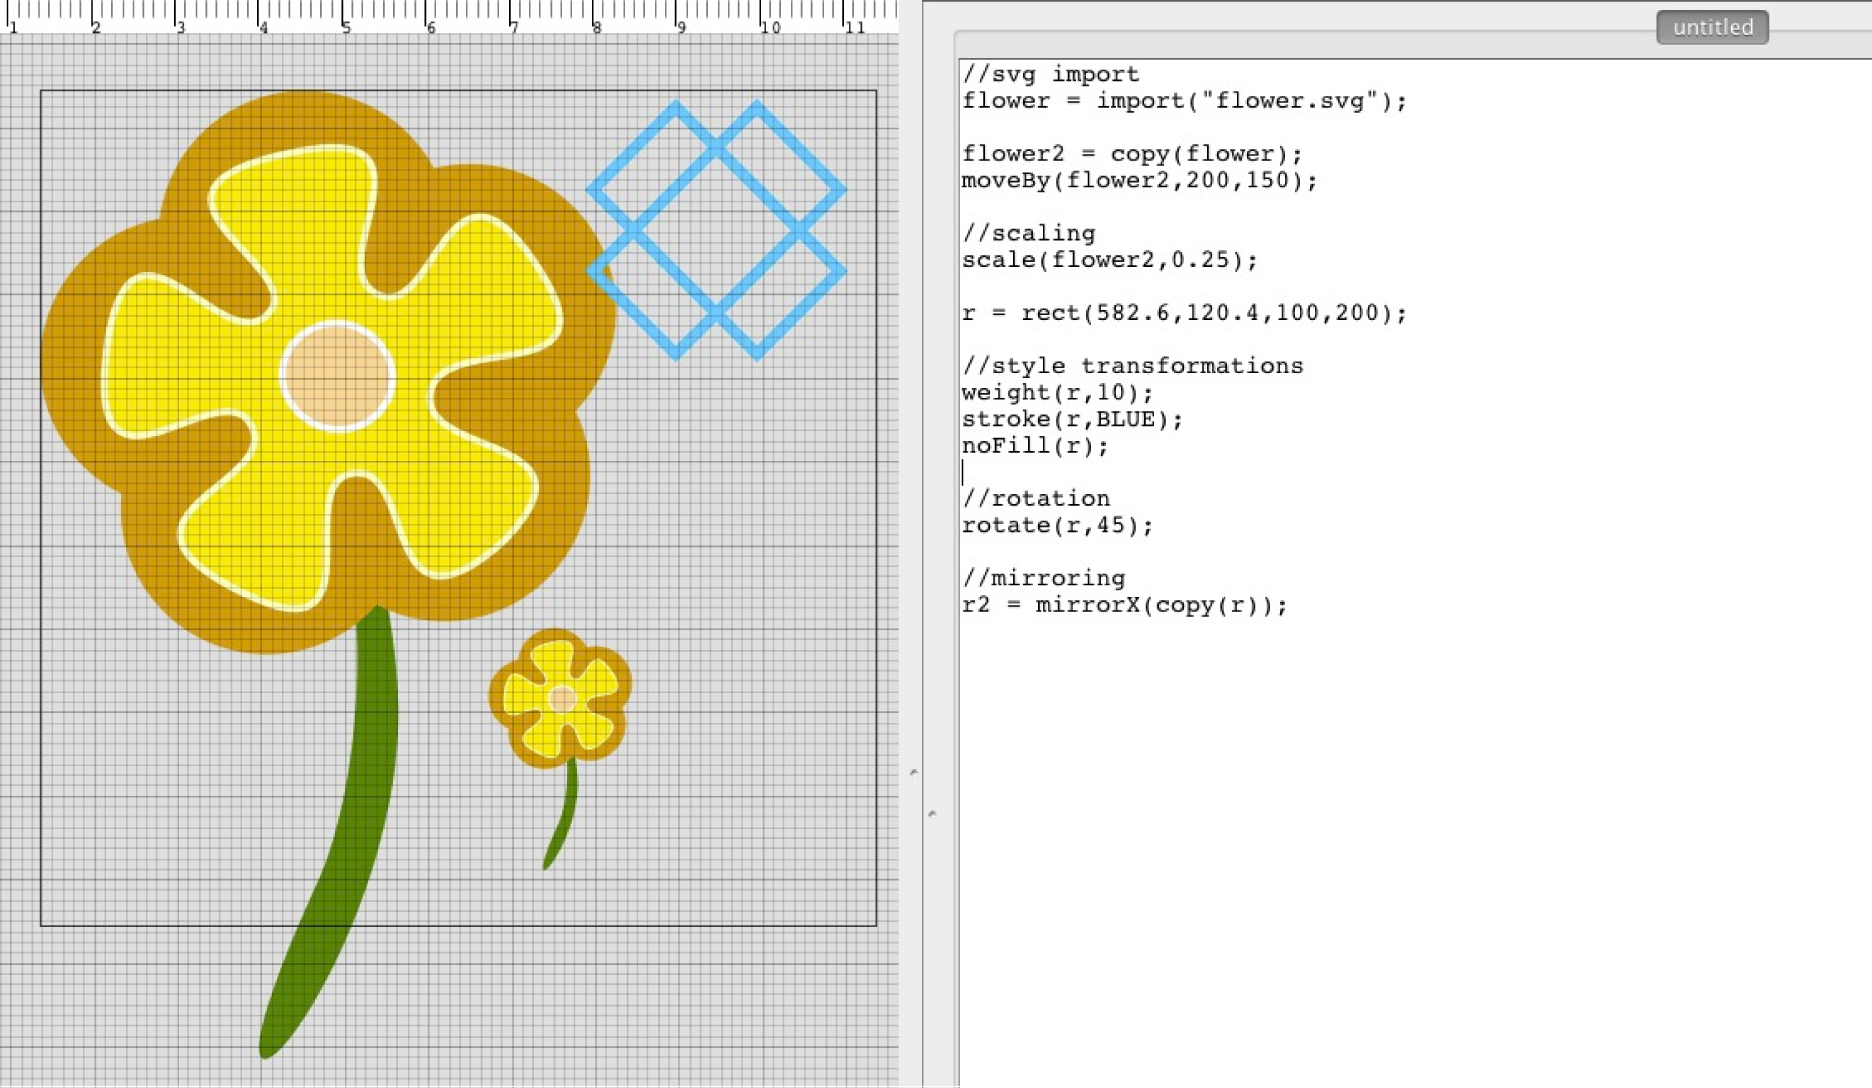
\includegraphics[width=6.5in]{images/transformation.png}
\caption{SVG import and sample of transformation methods}
\label{fig:transformation}
\end{figure}
\end{center} 

DressCode primitives can also be programmatically "grouped". Grouping provides an organizational structure for more complex configurations of primitives allows for the automatic transformations to multiple shapes. Groups have their own origin, which is used as the reference point for all move, rotation and scale methods applied to the group (figure: \ref{fig:grouping}.) For example, a collection of ellipses that is grouped and then moved to the center of the canvas would move the origin of the group to the center, and all the ellipses relative to the new origin. The origin of a group is automatically calculated as the centroid of all of the objects in the group and updated each time a primitive is added or removed. Groups are treated similarly to lists in that individual objects can be accessed and manipulated by via their index. Originally, primitives within a group were transformed relative to the origin of the group, however this caused confusion among many of our initial users. Each individual primitive is now translated according to the coordinate system of the canvas, regardless of whether it is in a group. 

 \begin{center}
\begin{figure}[h!]
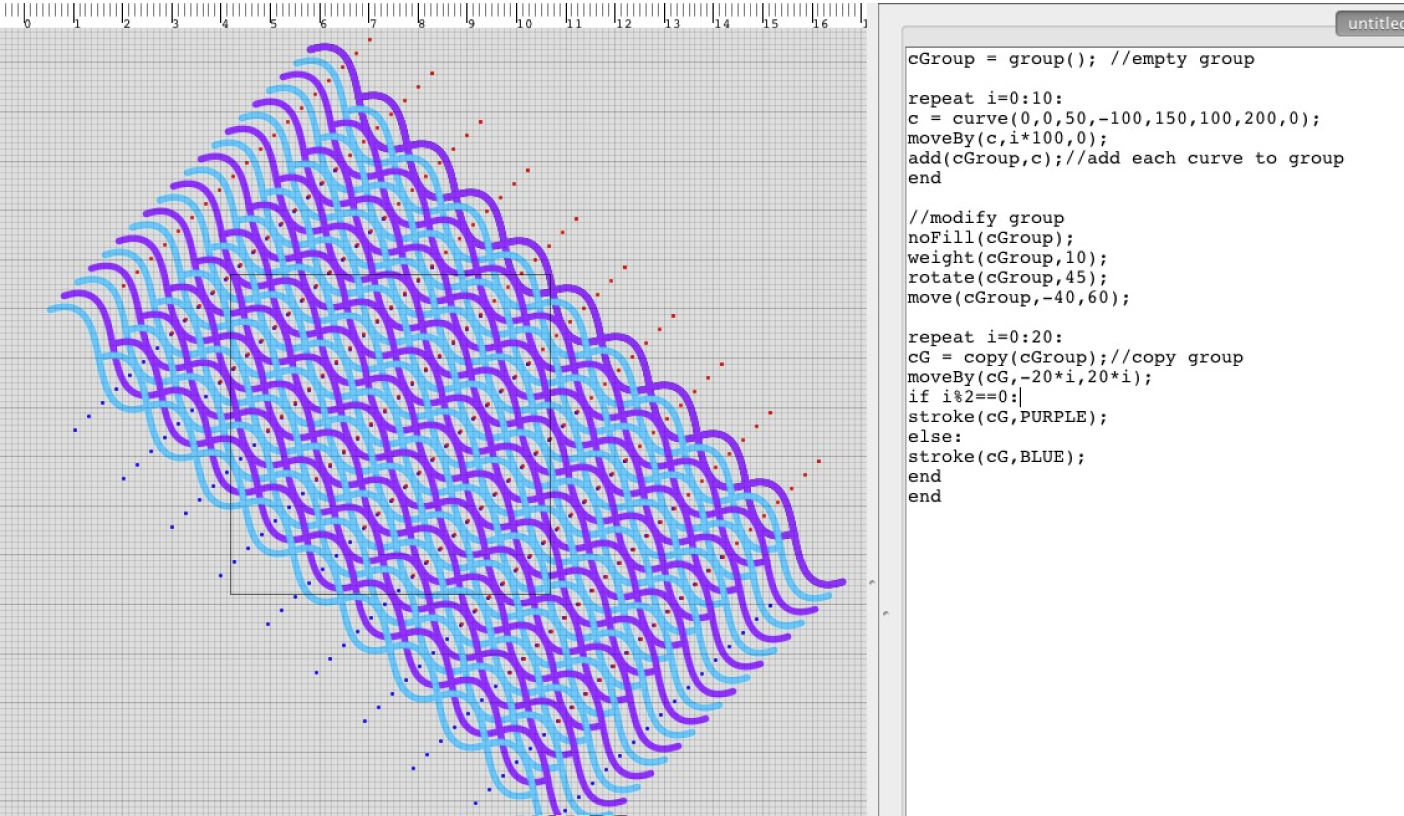
\includegraphics[width=6.5in]{images/grouping.png}
\caption{Grouping with transformation and repeat statements}
\label{fig:grouping}
\end{figure}
\end{center} 

\paragraph{Polygon Booleans:}
DressCode also features a subset of transformation methods for polygon boolean operations (figure: \ref{fig:boolean}.) The union, difference, exclusive or and intersection methods accept two primitives as arguments and return the corresponding shape, or group of shapes, depending on the operation. In addition, the merge method performs a union on all objects within a group and returns a single primitive. The expand method converts an object's stroke to a filled polygon with dimensions that match the weight of the stroke. The boolean methods were added for multiple reasons. Polygon boolean operations play an important role in CAD design for fabrication, because they allow for the creation of vector paths that appropriate for subtractive manufacturing processes. In particular, the merge method can function as a catch-all method for preparing designs for fabrication, and the expand method is useful for converting line drawings to paths that will retain their appearance when cut. In prior workshops, we relied on illustrator to prepare file paths for manufacturing, which was difficult, time-consuming and a hindrance to the computational design process. By integrating boolean operations as a part of the programming language in DressCode, it not only prevents users from having to rely on multiple software tools to design, but allows booleans to be used in a computational context, facilitating the creation of a whole new range of forms with simple primitives. 

Both the syntax and functionality of the boolean operations have been modified significantly since the first version of DressCode. In early versions, the majority of the booleans were expressed through mathematical notation, rather than with built in functions (e.g. ellipse1 + ellipse2 would perform a union). After some of our early user testing however, we depreciated this syntax, because many testers felt that mathematical notation was not intuitive beyond the union and difference operations. In addition, the mathematical notation required that all booleans be set equal to an identifier  (e.g. ellipse1 + ellipse2 = e3), in order to evaluate as a valid statement. The new method syntax still returns a resulting boolean, but can also be called without a corresponding assignment statement. Semantically, we originally had the boolean statements operate in a destructive manner as is the case in many graphic drawing programs; union(ellipse1, ellipse2) would destroy the original two ellipses and set the identifier ellipse1 equal to the resulting boolean. This was confusing however, because in a imperative program, the programmer could still reference the destroyed ellipse2. What we opted for instead, was a non-destructive boolean method wherein union(ellipse1,ellipse2) would return a third shape, which would automatically be drawn on the screen, and could be assigned to an identifier as needed. The original ellipse1 and ellipse2 would be hidden, but could both still be referenced without conflict, and could be revealed again on the canvas with the show() method. 

 \begin{center}
\begin{figure}[h!]
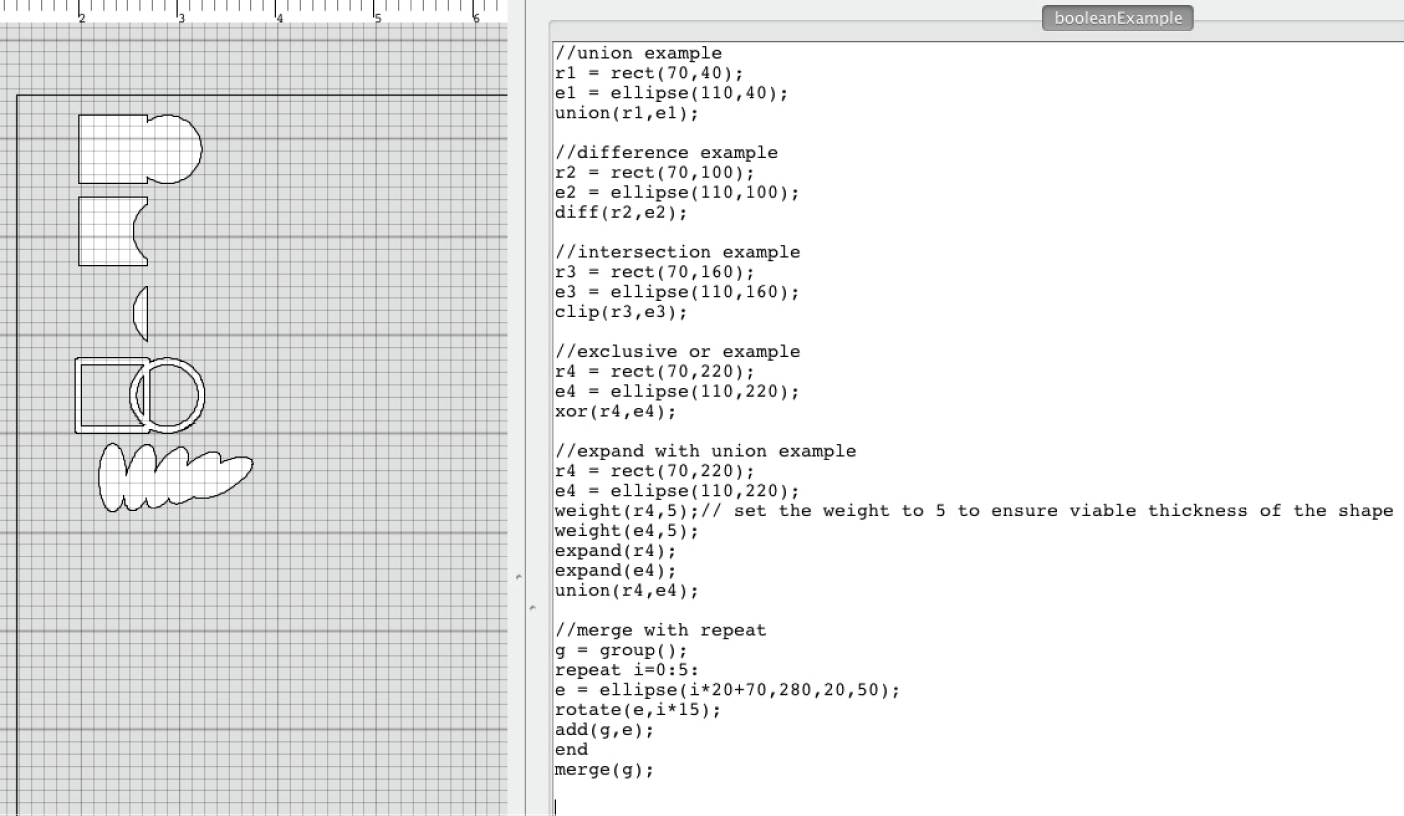
\includegraphics[width=6.5in]{images/boolean.png}
\caption{Polygon boolean operations}
\label{fig:boolean}
\end{figure}
\end{center} 
\paragraph{Additional Methods:}
Aside from methods for shape generation and transformation, DressCode features a set of getter methods that return information about a shape primitive, including its location, origin point, width and height, as well as a method to determine the Euclidean distance between two objects. There are also a set of methods that enable more advanced mathematical operations, including trigonometric functions, mapping, rounding and random number generation. The random method posses an interesting questions for implantation, as it generates different numbers each time a a program is run. This can be a useful design feature, allowing for the generation of numerous patterns with random variations. Figure \ref{fig:random_symmetry} demonstrates variations of an algorithm that produces randomly symmetrical stripe patterns.  It can also become problematic however, when the user wishes to keep the same randomly generated number for each interpretation of their program.  Finally, we recently added a set of methods that allow the specification of numerical values in inches, centimeters and millimeters, or in the current units of the drawing board. These methods are helpful when sizing and transforming primitives to real world measurements rather than pixel values.  

\paragraph{Constants:}
DressCode has a small set of constants to assist with design. WIDTH and HEIGHT correspond to the width and height of the current drawing board. PI corresponds to the numerical Pi value. Lastly, there are a set of color constants; RED, GREEN, BLUE, PURPLE, PINK, etc., that can be used to define the color of objects with fill and stroke methods. Custom colors can also be specified with 0-255 RGB values. 

 \begin{center}
\begin{figure}[h!]
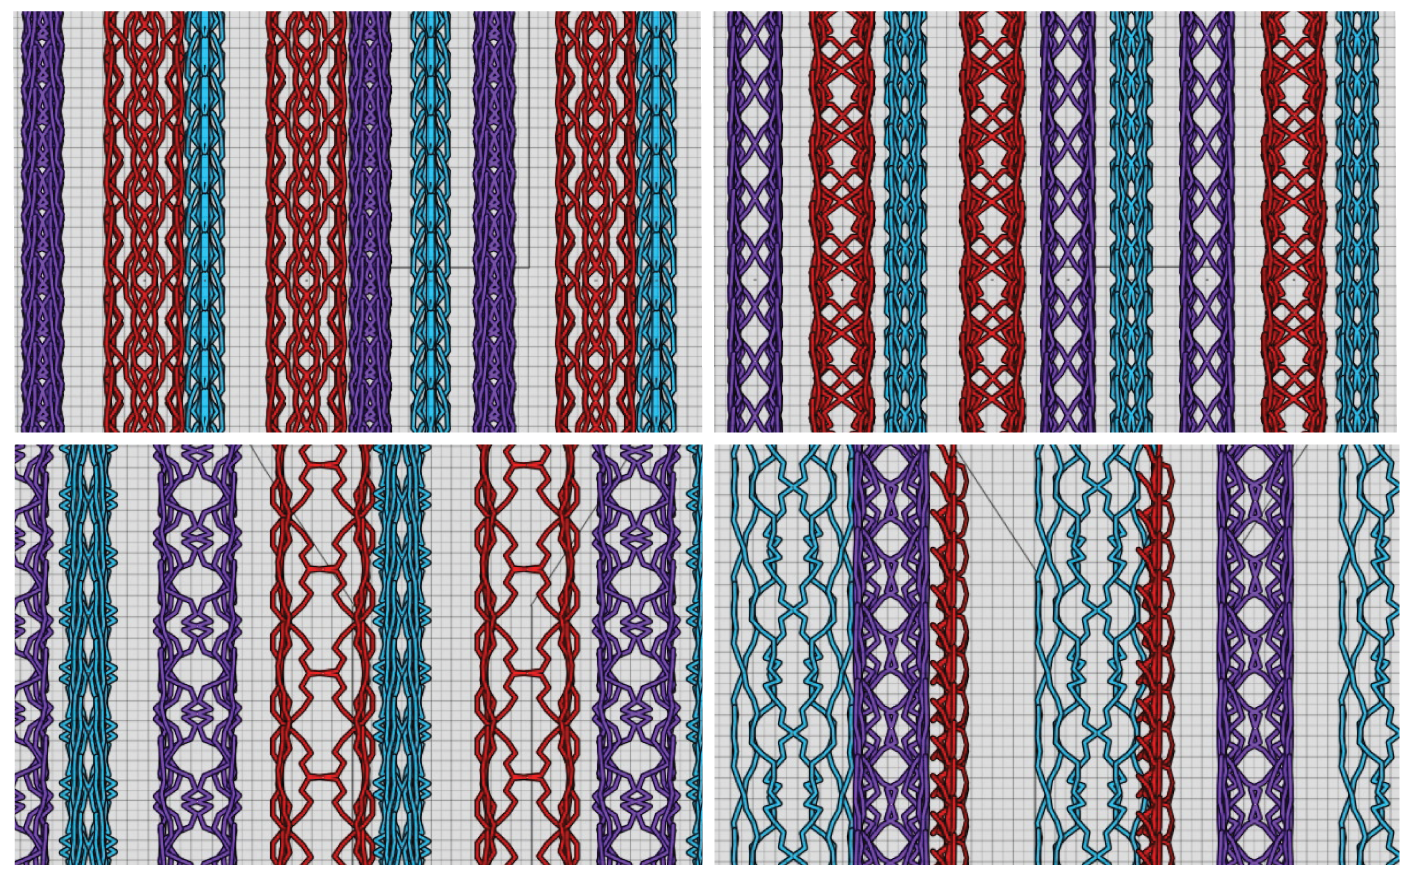
\includegraphics[width=6.5in]{images/random_symmetry.png}
\caption{Stripe pattern variations using the DressCode random method }
\label{fig:random_symmetry}
\end{figure}
\end{center}
